\chapter{Orchestrace kontejnerů}
Ochestrátory vznikly jako odpověď na rozšiřování kontejnerové virtualizace. Kontejner má stejný problém jako VM, bez orchestrace je práce s nimi velmi zdlouhavá a neefektivní. Na rozdíl od klasické virtualizace se ve světě mikroslužeb pracuje se stovkami tisíc až milióny kontejnerů a tyto objekty je potřeba ovládat. Orchestrátory slouží ke správě a ovládání kontejnerů, pomocí nich lze škálovat, rozdělovat zdroje a řešit spoustu problémů, které by se bez jejich použití musely řešit manuálně. Jak vyplývá z prezentace zaměstnance Google Joe Beda americký internetový gigant Google\cite{beda_prez} spouští během každého týdne cca na 2 miliardy nových kontejnerů. Takové množství nelze spravovat bez orchestrátoru. 

Pro dnešní typy kontejnerů existuje na trhu řada orchestrátorů jejíž vývoj kopíruje vznik Dockeru, ale první stabilní verze 1.0 byly vydávány v letech mezi 2015 a 2016\cite{docker_1_0}. Všechny tyto nástroje jsou taktéž jako kontejnerové technologie open source.

Orchestrátory fungují na jednoduchém principu, rozdělují jednotlivé kontejnery do logických skupin a pracují se skupinou samostatně, například  skupina pro webové servery, databáze atd. Díku tomuto faktu lze pak s logickou skupinou pracovat jako s jedním kontejnerem. Například v případě potřeby přidání  storage se připíše její definice pouze k předpisu pro tuto skupinu a orchestrátor zajistí, že všechny kontejnery dostanou potřebné místo.

Networking v rámci orchestrátorů je velmi odlišný od Docker networkingu. Každý orchestrátor má v základu své řešení, které většinou dovoluje komunikovat veškerým kontejnerům navzájem mezi sebou, což není optimální ve všech případech. Pokud běží na jedné infrastruktuře více odlišných aplikací, pak je nutno omezit jejich viditelnost. Problémy, které jsou v rámci síťování potřeba vyřešit jsou následující: komunikace mezi kontejnery, viditelnost vůči externímu světu a vysoká dostupnost\cite{K8S_micro}. Podobně, jak je tomu u klasické virtualizace, existují i projekty od externích firem, které rozšiřují a vylepšují základní koncept networking u orchestrátorů a přidávají spoustu nových funkcí (OpenContrail, Calico, Romana, apod.).

Pro nasazení kontejnerů v produkčním prostředí je potřeba vyřešit ještě mnoho důležitých otázek a požadavků, které jsou od těchto prostředí vyžadovány. Spousta vlastností jako vysoká dostupnost či life cycle managment nejsou pouze o vybrané technologii, ale i o designu daného prostředí. Pokud je navrženo špatně, tak vybrané technologie nemohou být využity efektivně. 

\section{Vysoká dostupnost} \label{par:ha}
Pojem vysoká dostupnost (v angličtině High Avalibility) popisuje proces, pomocí kterého se udržuje infrastruktura dostupná pro uživatele. Pokud má infrastruktura tento prvek správně navržený, koncový uživatel by neměl poznat žádný problém způsobený například pádem databáze nebo webového serveru. Faktor vysoké dostupnosti bývá někdy podceňován, nejedná se totiž jenom o infrastruktru, ale i o datacentra, kde se daná infrastruktura nachází. Vysoká dostupnost závisí na čtyřech hlavních kategoriích hardwaru, sítí, storage a používaného softwaru. Cílem vysoké dostupnosti je omezit tzv. single point of failure, jedná se o jednu část, například službu, při jejímž výpadku by mohlo dojít k poruše celého prostředí.

Řešení problému single ponint of failure probíhá pomocí mnoha procesů, které slouží jako prevence před případným výpadkem prostředí. Důležité je duplikovat služby a pokud je to možné, provozovat je v cluster módu, aby případný výpadek jedné komponenty v clusteru nemohl ovlivnit zbytek. Velmi důležitou částí v tématu vysoké dostupnosti hrají load balancery, které slouží pro rozložení zátěže mezi více odlišných a na sobě nezávislých komponent, například webserver, viz obrázek \ref{fig:load_balancing}. Je potřeba zmínit, že pokud se na produkční prostředí přistupuje prostřednictvím load balanceru, je nutné vytvořit z load balancerů cluster, a tím zamezit případným výpadkům prostředí.

\begin{figure}[H]
\begin{centering}
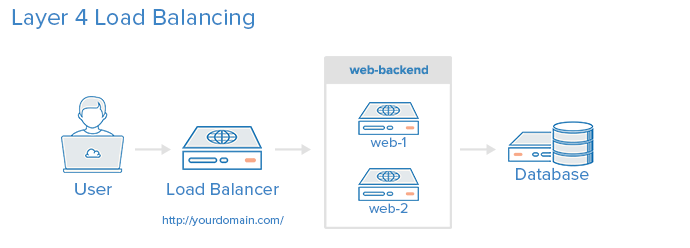
\includegraphics[width=1\textwidth]{img/load_balancing}
\par\end{centering}
\caption{Ukázka architektury Load Balanceru, převzato z: \cite{lb_ha} \label{fig:load_balancing}}
\end{figure}

V produkčním prostředí jsou požadavky na dostupnost služeb velmi vysoké, proto je nutno aplikovat pravidla pro vysokou dostupnost. Pomocí implementací principu vysoké dostupnosti lze minimalizovat výpadky v prostředí. Moderní programy zaměřující se na řešení vysoké dostupnosti provádějí i automatické obnovy ze záloh serveru či dokonce obnovu chybných komponent v clusteru. 

\section{Škálovatelnost}
Dalším faktorem, který je nutno při výběru orchestrátoru třeba zvážit, je škálovatelnost neboli schopnost rozšiřovat dané prostředí. V dnešní době se stává, že firmy rostou několikanásobně za rok. V důsledku přibývajících uživatelů a jejich potřeb je nutno škálovat a rozšiřovat dané služby tak, aby byla uspokojena uživatelská poptávka. S tímto problémem se například potýká největší poskytovatel streamované hudby na světě server Spotify.
Ve škálovatelnosti jsou definovány dva základní druhy škálování, a to horizontální a vertikální. Vertikální prostředí můžeme chápat jako přidávání dalších zdrojů pro hardware, přidávání disků a rozšiřování RAM. Škálování horizontální je rozšiřování daných služeb na jedné infrastruktuře.

Orchestrátory umí škálovat pouze horizontálně. Hlavním parametrem škálovatelnosti je čas, za který orchestrátor vytvoří nové kontejnery, a tím zvýší dostupnost stávajícím službám. Obdobný princip funguje i obráceně. Pokud není potřeba zpracovávat velké množství dat od koncových uživatelů, je možno kontejnery s těmito nepoužívanými aplikacemi jednoduše zastavit. 

Ochestrátory mohou provádět škálování kontejnerů automaticky podle nastavených specifik, prostředí se  automaticky přizpůsobuje potřebám aplikací a není tak nutný manuální zásah administrátorů přímo do prostředí.

\section{Life cycle managment}
Life cycle managment (LCM) je založen na řadě procesů, které slouží  k udržování a běhu aplikace po dobu produkce. Infrastruktura je živé prostředí, ve kterém je doporučeno uchovávat a spravovat konfigurační soubory.
V rámci automatizace těchto kroků vznikla nová sada nástrojů spadající do skupiny konfigurační management. Pomocí těchto nástrojů lze vzdáleně přes jeden server ovládat stovky až tisíce serverů. Mezi tyto nástroje patří Ansible, Puppet, SaltStack, Chief atd.
Globální konfigurační soubory je vhodné ukládat přes distribuovanou službu, například git. Konfiguraci je  vhodné verzovat a mít tak možnost vrátit se ke starším verzím konfiguračních souborů. Užitečná vlastnost na verzovacích nástrojích je kontrola změn. Všechny verze se změnami konfigurace se ukládají do repositářů. Pokud je repositář, ve kterém jsou uloženy konfigurační soubory správně nastaven, není možné, aby nikdo z administrátorů, který upravuje konfiguraci, změnil historii repositáře. Další výhodou těchto nástrojů pro distribuovanou správu verzí je indexování změn.
V LCM je velmi důležité téma aktualizace stávajících aplikací běžících v kontejnerech. V rámci prudkého vývoje aplikací je velmi důležité nasazení nové verze do produkce velmi rychle. 

\section{Typy orchestrátorů}
Na trhu existuje mnoho projektů na správu kontejnerových prostředí. Tato práce se zaměřuje na pět základních druhů. Orchestátory se převážně liší svým přístupem a ovladatelností, ne všechny jsou vhodné jako produkční orchestrátory ve velkých infrastrukturách. U jednotlivých technologií je rozhodující počet kontejnerů, se kterými orchestrátor dokáže pracovat.

\subsection{Docker Compose}
Compose je řešení od firmy Docker, které zajišťuje spouštění multi-kontejnerových Docker aplikací. Lze ho označit jako jednoduchý orchestrátor. Na rozdíl od ostatních řešení nabízí poměrně málo funkcionality. Hlavním stavebním kamenem služby Compose je konfigurační yml dokument, pomocí kterého se nastavuje spojení mezi jednotlivými kontejnery. Do logických bloků se nadefinují potřebné údaje jako jsou image, volume, které je pro dané prostředí nutné nastavit. Vzorová ukázka Docker Compose souboru v yml formátu se nachází v ukázce kódu číslo \ref{lst:compose_code}.  Dalšími přednostmi yml je čitelnost a přehlednost, která je u formátu json  horší. 

Velká přednost, a zároveň nevýhoda tohoto řešení, je jeho jednoduchost. Tento koncept je spíše použitelný zejména pro vývojáře, kteří si mohou pomocí Compose spustit jednoduché vývojové prostředí s předem nadefinovanými službami (databáze, webserver, apod.). Compose vůbec neřeší problém jako jsou vysoká dostupnost, distribuovanost a LCM, proto není vhodný pro velké infrastruktury.  

\begin{lstlisting}[caption={Docker Compose pro Wordpress s MySql databází},label= {lst:compose_code}]
version: '2'
services:
   db:
     image: mysql:5.7
     volumes:
       - db_data:/var/lib/mysql
     restart: always
     environment:
       MYSQL_ROOT_PASSWORD: wordpress
       MYSQL_DATABASE: wordpress
       MYSQL_USER: wordpress
       MYSQL_PASSWORD: wordpress

   wordpress:
     depends_on:
       - db
     image: wordpress:latest
     ports:
       - "8000:80"
     restart: always
     environment:
       WORDPRESS_DB_HOST: db:3306
       WORDPRESS_DB_PASSWORD: wordpress
volumes:
    db_data:
\end{lstlisting}

\subsection{Fleet}
Fleet je další z projektů od firmy  CoreOS. Je založen na systemd. Systemd nyní používá většina Linuxových distribucí jako init a pomocí něj spravuje procesy\cite{fleet_systemd}. Fleet by se dal nazvat jako systemd pro cluster, který si udržuje data v distribuované databázi etcd. Tento projekt směřuje primárně na linuxovou distribuci od firmy CoreOS Container Linux. Práce s clusterem je jednoduchá, velmi podobná práci se systemd samotným. Samostatné používání tohoto orchestrátoru na velkém produkčním prostředí je trochu limitující, sami autoři projektu nedoporučují použít Fleet na více jak 100 serverech s více než 1000 službami\cite{fleet_lim}. V únoru 2017 firma CoreOS pozastavila vývoj uvedeného orchestrátoru a začala ve všech svých produktech používat Kubernetes\cite{fleet_end}. 

\subsection{Docker Swarm}
Swarm je nástroj pro tvorbu clusteru pro Docker kontejnery. Původně byl doručován jako doplněk k Docker kontejnerům. Od verze Dockeru 1.12 byl přidán do stejného balíku\cite{docker_1_12}, ve kterém je doručováno kontejnerové řešení. V tomto novém řešení přišel s vlastnostmi a architekturou velmi podobnou konkurenčnímu řešení Kubernetes, viz obrázek \ref{fig:swarm_arch}. Swarm má k dispozici vlastnosti jako rolling update, decentralizovaný design, multi-host networking, load balancing. Jednou z výhod tohoto řešení je nativní podpora pro spouštění již předvytvořených Compose souborů\cite{swarm_compose}. 

V porovnání s Compose se jedná už o vyspělejší řešení podobné ostatním orchestrátorům. Nabízí v základu mnoho vestavěných funkcí. Jeho možnosti jsou stále omezené ve srovnání s komunitou a ekosystémem okolo Kubernetes. Swarm řešení je vhodné pro malé clustery, je velmi jednoduché na operování, nasazení a použitelné v malých produkčních prostředích. Jednou z limitací  orchestrátoru Swarm je rozšiřitelnost, dokáže pracovat pouze s Docker kontejnery. 


\begin{figure}[H]
\begin{centering}
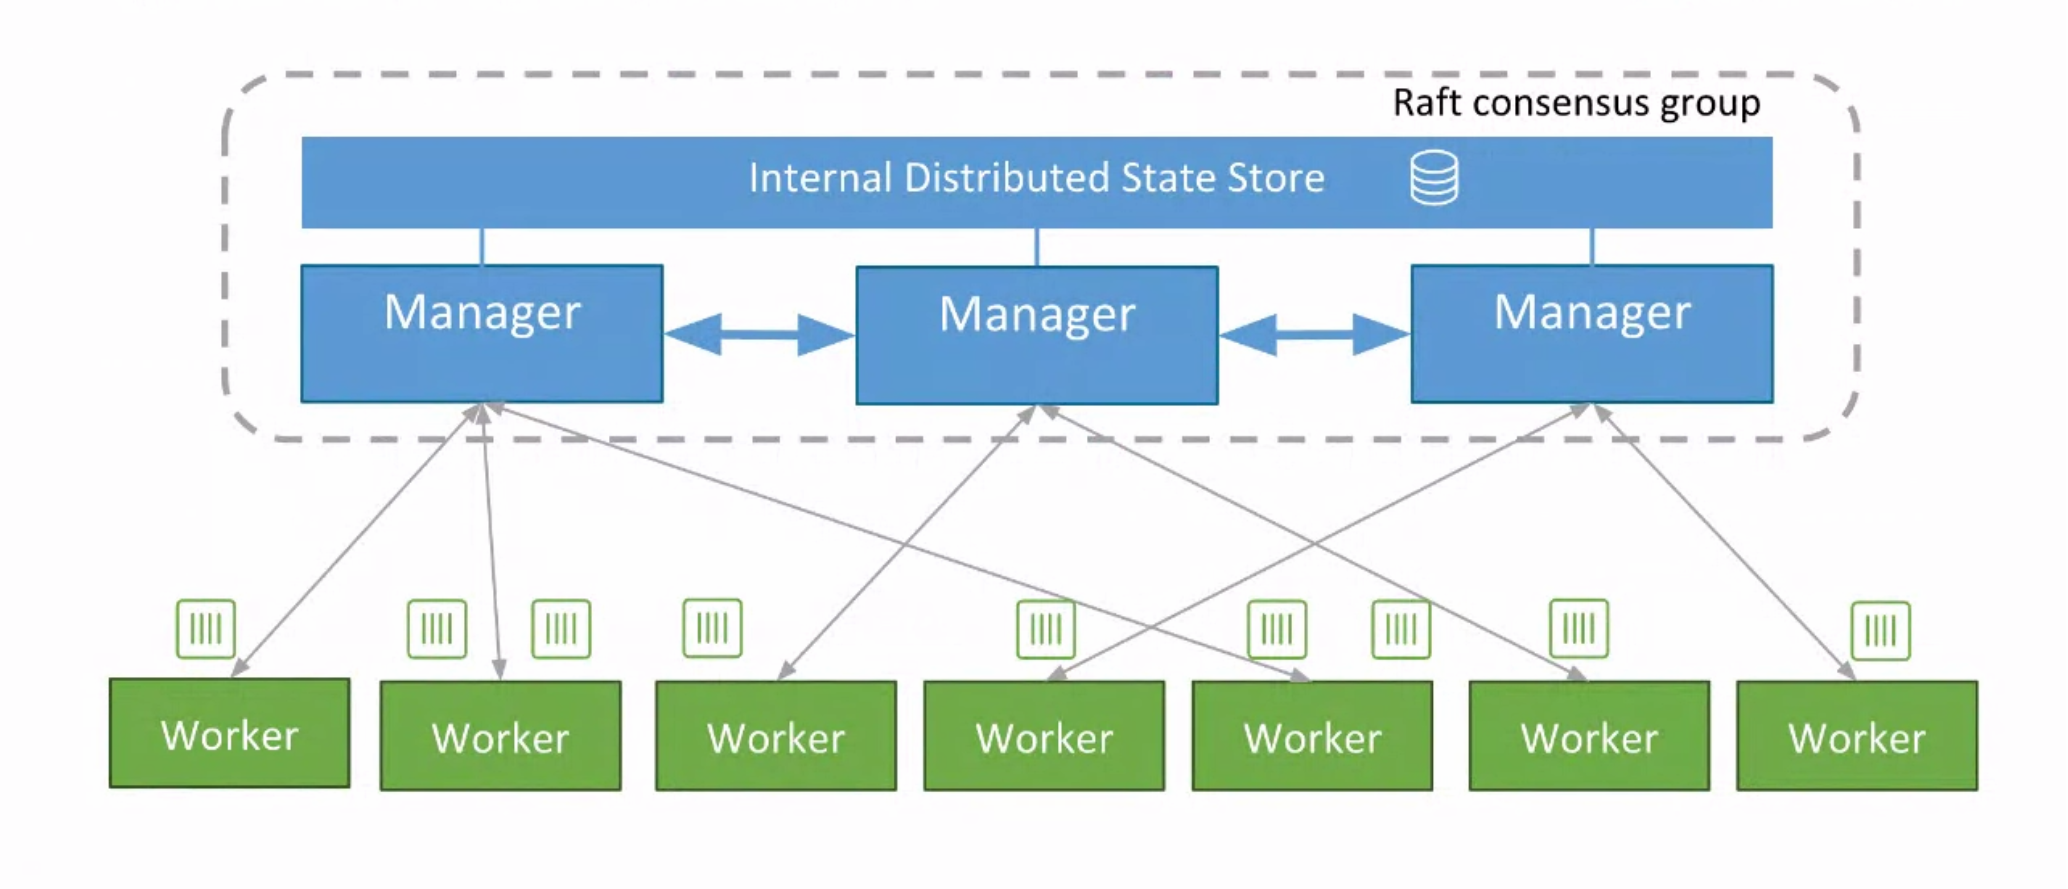
\includegraphics[width=1\textwidth]{img/swarm_arch}
\par\end{centering}
\caption{Docker Swarm architektura, převzato z: \cite{swarm_arch} \label{fig:swarm_arch}}
\end{figure}

\subsection{Apache Mesos}
Apache Mesos je projekt, který se zabývá problematikou distribuovaných clusterů. Od ostatních orchestrátorových řešení se Mesos liší tím, že se nezaměřuje pouze na kontejnery. Pracuje převážně s hardwarovými zdroji, byl vytvořen už v roce 2009 na Univerzitě v Berkeley v Kalifornii\cite{mesos}, a to o tři roky dříve než se začaly objevovat první verze kontejnerů od Dockeru. Je sestaven převážně z projektů pocházejících z Apache Foundation, viz obrázek \ref{fig:mesos_arch}. Jedná se o open source řešení.

Hlavní odlišností od Kubernetes a Swarmu je dvou-úrovňový scheduler, který na první vrstvě pracuje se zdroji pomocí různých typů labelů. Jimi lze odlišovat a spojovat do skupiny různé tipy hardwarových zdrojů. Na druhé vrstvě scheduleru Mesos rozděluje zdroje mezi zdrojové frameworky a frameworky s technologií běžící v nich. Na spouštění kontejnerů pak slouží Marathon framework.

Tento orchrestrátor se často porovnává s open source řešením pro cloud computing OpenStack. Mesos také bývá používán na řešení problematiky velkých objemů dat. 

\begin{figure}[H]
\begin{centering}
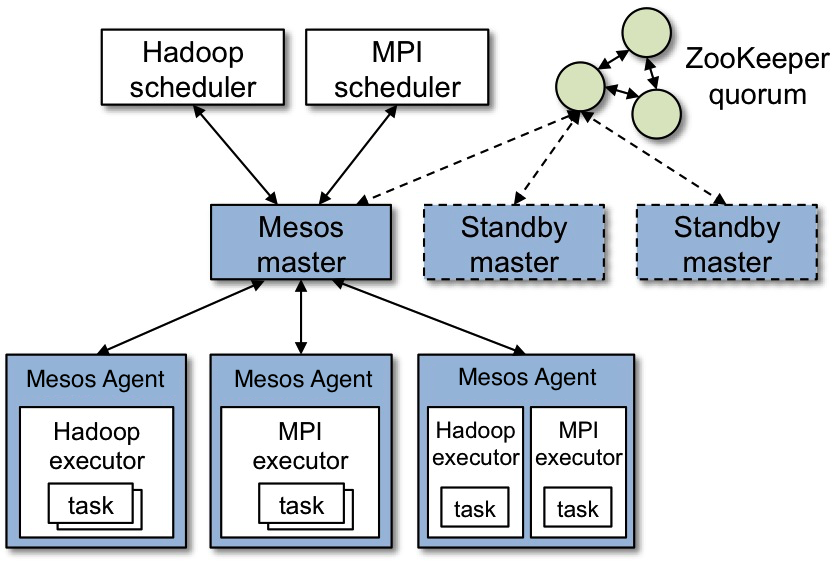
\includegraphics[width=1\textwidth]{img/mesos_arch}
\par\end{centering}
\caption{Mesos architektura, převzato z: \cite{mesos} \label{fig:mesos_arch}}
\end{figure}

\subsection{Kubernetes}
Projekt Kubernetes pochází od firmy Google, tato americká firma používá v produkčním prostředí výhradně kontejnerové technologie\cite{beda_prez}. Všechny jejich webové služby jsou spuštěny v tomto typu virtualizace. Kubernetes je orchestátor, který na rozdíl od ostatních technologií podporuje více kontejnerových řešení. Dokáže pracovat s většinou kontejnerových technologií, jako je Docker, rkt, crio-o, Windows kontejnery atd. Kubernetes by se dal nazvat spíše frameworkem než orchestrátorem, je na rozdíl od ostatních řešení velmi modulární a existuje pro něj celá řada rozšiřujících modulů\cite{k8s_kuba}. 

Kubernetes umožňuje spouštět a spravovat kontejnery, nezávisle na hardware Kuberenetes si sám vybírá místo pro spuštění kontejnerů. Podobně jako u Mesosu řadí všechny fyzické zdroje do jednoho celku, ze kterého si podle potřeby postupně alokuje zdroje. 

Kubernetes se skládá ze dvou základních rolí, master a node (dříve nazýván minion). Master je hlavní součást, která kontroluje jednotlivé skupiny nodů. Nody přebírají požadavky od mastera a vykonávají  akce stanovené masterem. Na základně provedené akce vracejí masterovi zpětnou vazbu o výsledku provedené akce. Kubernetes pro spouštění a správu kontejnerů používá tři základní komponenty: pod, replication controller a Kubernetes services a kubelet viz obrázek \ref{fig:kube_arch}.

Pod je základní stavební jednotka Kubernetes. Jednotlivé kontejnery jsou umísťovány do těchto na sobě nezávislých podů, které nejsou závislé na hostiteli. Do jednoho podu je možno uložit celou aplikaci, která se skládá z více na sobě závislých kontejnerů. Velká výhoda toho konceptu je následná práce s pody, se kterými lze pracovat jako s celistvým objektem. K podu lze připojovat různé zdroje, které mohou kontejnery uvnitř sdílet. 

Replication controller hlídá a definuje pody. V Kubernetes se používá při horizontálním škálování. Další důležitá funkcionalita replication controlleru je hlídání stávajících podů a kontejnerů v nich. V případě výpadku podů nebo výpadku hostitelského stroje, na kterém pod pracuje replication controller je schopen zmonitorovat a spustit nový pod na jiném hostu. V případě, že je chyba na jednom hostu, jsou všechny jeho pody spuštěny na jiném stroji. Pokud je původní host obnoven, pody se opět vrátí na původní místo a stávající pody jsou zrušeny.

\begin{figure}[H]
\begin{centering}
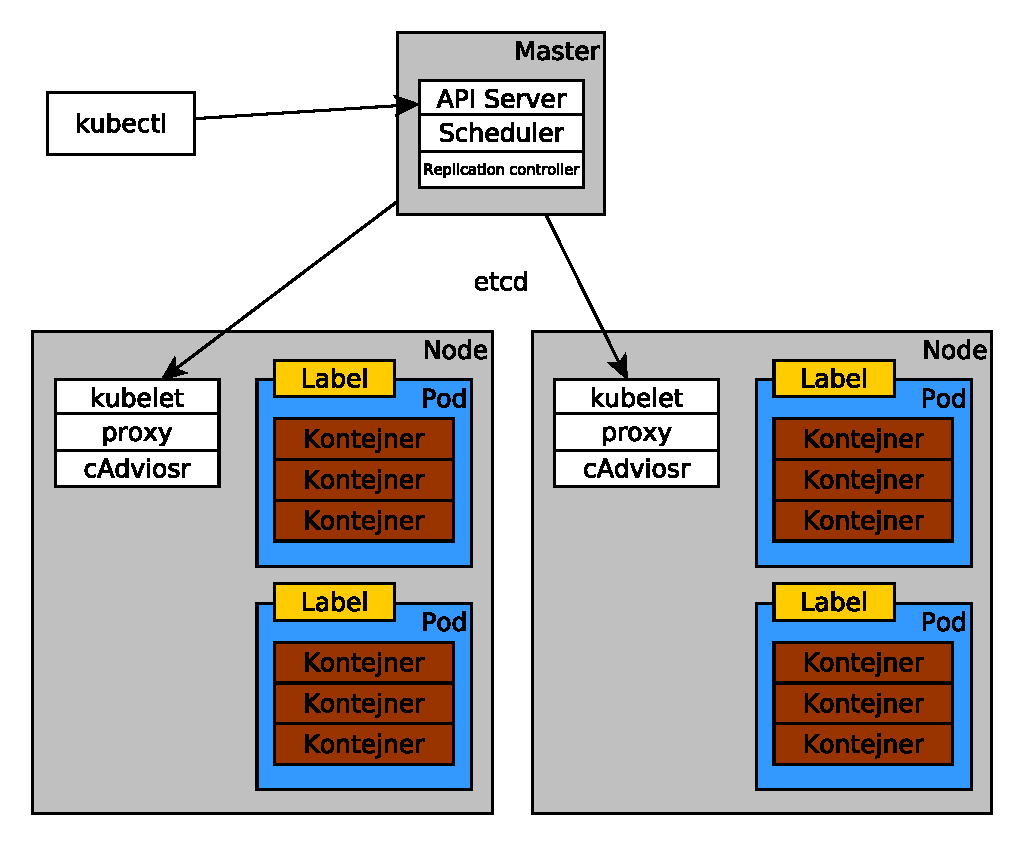
\includegraphics[width=1.0\textwidth]{img/kubernetes}
\par\end{centering}
\caption{Kubernetes architektura, zdroj: vlastní tvorba \label{fig:kube_arch}}
\end{figure}

\section{Porovnávání orchestrátorů}
Z porovnání jednotlivých orchestračních nástrojů lze vysledovat, že většina z nich implementuje maximálně dvě řešení pro spouštění odlišných tipů kontejnerů. Všechny orchestátory až na fleet lze spustit na odlišných platformách, nutno zmínit, že nativní podporu má pouze Linux. Konkurenční platformy jako Mac a Windows lze využít pouze na testování nebo vývoj aplikací pro tyto orchestátory. Škálovatelnost jako hlavní prvek a účel orchestrátoru je podporována napříč všemi vybranými řešeními.  Postupy pro řešení failoverů a vysoké dostupnosti jsou implementovány taktéž u většiny řešení. Pokud je nutné pro orchéstrátor využít externí rozšiřující doplňky pro síťování, je výběr velmi omezen. Tuto funkcionalitu podporují pouze tři řešení, z toho Docker Swarm, podporuje jen jednoduchá SDN. Pokročilé SDN nástroje jako OpenContrail, pomocí kterých lze Kubernetes integrovat do stávajících virtualizačních platforem jako je OpenStack jsou dostupné pouze pro Mesos a Kubernetes. Srovnání orchestrátorů je uvedeno v tabulce \ref{tbl:orch_comp}.

\begin{table}[H]
\begin{center}
\caption{Porovnání orchestrátorů}
\label{tbl:orch_comp}
\begin{tabular}{|c|c|c|c|c|c|}
\hline
  ~   & Compose & Swarm & Fleet & Mesos  &  Kubernetes \\    \hline
Kontejnery          &  Docker &  Docker & Docker, rkt &  Docker, rkt &  \makecell{ Docker, rkt,\\cri-o, \\Windows Containers}  \\    \hline
Škálovatelnost &  Ano &  Ano & Ano &   Ano & Ano \\    \hline
Failover &  Ne & Ano & Ano &  Ano & Ano \\    \hline
Vysoká dostupnost &  Ne  &  Ano & Ano &   Ano & Ano \\    \hline
Netowkring pluginy &  Ne &  Ano & Ne &   Ano & Ano \\    \hline

\end{tabular}
\end{center}
\end{table}

